
\chapter{Technische uitvoering}

%Een beschrijving van de technische uitvoering van het project met de
%nodige figuren en een verantwoording van de ontwerpskeuzes.

% Structuur:
% Waarom
% Voornadelen / nadelen
% Werking
Triump bestaat uit twee grote delen. Enerzijds is er de frontend, dit is het gedeelte van Triump waarmee de gebruikers rechtstreeks intrageren. De frontend bestaat op zijn beurt uit twee delen, nl. een Android applicatie en een webinterface. Het tweede deel van de Triump infrastructuur is backend. Hiermee komen de gebruikers nooit rechtstreeks in contact. In onderstaande paragrafen wordt er dieper ingegaan op deze onderdelen. Figuur \ref{fig:algemene structuur backend} geeft een abstract overzicht van de infrastructuur.
\begin{figure}[H]
	\centering
	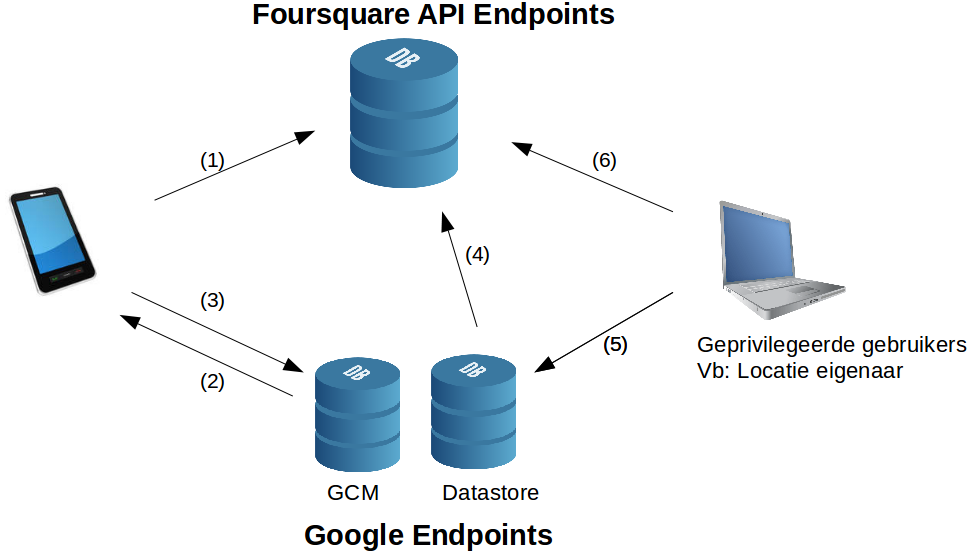
\includegraphics[scale=0.3]{backend_algemene_structuur}
	\caption{Structuur backend}
	\label{fig:algemene structuur backend}

\end{figure}

\section{Backend}

\subsection{Google Cloud Endpoints}
\label{sec: GCE}
% restricities op aantal request
Google Cloud Endpoints (GCE) is een uitbreiding van Google App Engine (GAE). GAE is een bekend "Platform as a Service" gemaakt om applicaties uit te voeren op de infrastructuur van Google. GCE biedt naast de functionaliteiten beschikbaar in GAE een extra infrastructuur om op een relatief eenvoudige manier een backend API te generen. 
De extra infrastructuur aangeboden door GCE bestaat uit de endpoints. Deze endpoints verzorgen ondermeer de communicatie en authenticatie tussen mobiele gebruikers en de backendserver.
Aangezien de backend API nog steeds gehost wordt door Googles App Engine blijven alle functionaliteiten zoals "Datastore", "Google Cloud Messaging" en "Cron jobs" beschikbaar. Figuur \ref{fig:Architectuur Google Cloud Endpoints} geeft de architectuur van de Enpoint weer~\cite{Google_endpoints}.

\begin{figure}[H]
	\centering
	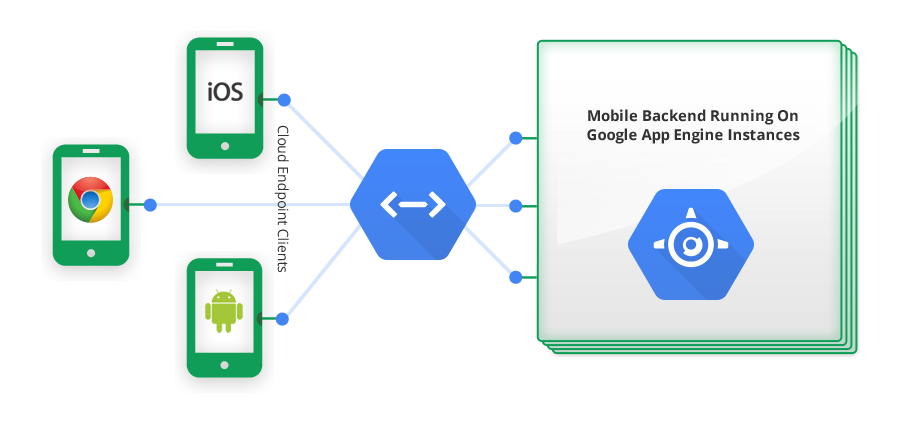
\includegraphics[scale=0.3]{GCE}
	\caption{Architectuur Google Cloud Endpoints}
	\label{fig:Architectuur Google Cloud Endpoints}
\end{figure}

Het voornaamste voordeel van het werken met GAE is dat er tijdens ontwikkelfase geen rekening hoeft gehouden te worden met het  beheer en de administratie van de backend infrastructuur. Problemen zoals schaalbaarheid worden via dynamische rekenkracht allocatie opgelost. Daarnaast verzekert de App Engine een permanente beschikbaarheid van de servers worden doorgeschoven.

Desalniettemin brengt het gebruik van GAE meerdere nadelen met zich mee. De voornaamste zijn de restrictie op het aantal lees- en schrijfoperaties per dag, de sterk variërende duratie van lees- en schrijfoperaties en de afhankelijkheid van een externe organistatie. Aangezien elke nieuwe ontwikkelaar \$ 300 cadeau krijgt kon het eerste nadeel opgelost worden door het aantal operaties per dag van 50.000 naar 1.000.000 te verhogen. De reden waarom 1.000.000 operaties per dag noodzakelijk is om Triump draaiende te houden is dat elke entiteit binnen een query als één leesoperatie wordt beschouwd. Hierdoor neemt het aantal leesoperaties bij het uitvoeren van enkele geneste queries zeer snel toe.

\subsubsection{Datastore}

Triump maakt gebruik van App Engine Datastore als backend databank.

GAE Datastore verschillend van traditionele relationele databases door zijn specifieke architectuur. De database is namelijk zo ontworpen dat het automatisch meeschaalt met de toenmende hoeveelheid opgeslagen data. Een tweede verschil met relationele databanken is dat GAE Datastore schemaloos is. Hiermee wordt bedoeld dat objecten van een eenzelfde type verschillende eigenschappen kunnen hebben en dat eenzelfde eigenschap verschillende types kan hebben. 

Objecten in de database worden entiteiten genoemd. Een entiteit heeft meerdere eigenschappen, elk van deze eigenschappen kan één of meerdere waarden hebben. 

Aangezien de database schemaloos is en bijgevolg bijvoorbeeld geen types zal controleren of niet zal aangeven indien een vreemde sleutel niet bestaat ligt de verantwoordelijkheid van de in integriteit van de database volledig bij de ontwikkelaar. Tijdens de ontwikkeling werd dit gezien als het grootste nadeel van de GAE Datastore.

\subsubsection{Google Cloud Messaging}
% Notificaties
%https://developer.android.com/index.html
Google Cloud Messaging (GCM) voor Android is een dienst die het mogelijk maakt data (tot 4kB) te versturen van backend servers naar Android smartphones. De GCM servers staat in voor de connectie naar het mobiele toestel en een correcte aflevering van de berichten.

GCM wordt in Triump gebruikt als basis van het notificatie systeem. In de huidige implementatie ontvangt een gebruiker een notificatie indien hij of zij een promotie of event heeft gewonnen en bijgevolg een prijs heeft verdiend. Principieel werkt het systeem als volgt:
\begin{enumerate}
  \item Een gebruiker heeft een prijs gewonnen.
  \item De backend construeert een korte boodschap. De boodschap en gebruiker die de boodschap dient te ontvangen wordt doorgegeven aan de GCM dienst. 
  \item GCM dienst verstuurd de booschap naar het mobiele Android toestel.
  \item Op het toestel draait een permanente service die luistert naar binnenkomende boodschappen. De ontvangen boodschappen worden omgevormd tot een notificatie.
  \item De notificaties worden weergegeven op het toestel.
\end{enumerate}
Pijl (2) van figuur \ref{fig:algemene structuur backend} geeft aan dat er via GCM, vanop de backend servers, berichten worden gepusht naar de gebruikers.
\subsubsection{Cron jobs}

Een van de functionaliteiten die Google App Engine aanbiedt is de App Engine Cron Service. Deze service laat gebruikers toe bepaalde taken (cron jobs/chronical jobs) op regelmatige tijdstippen uit te laten voeren op de backend. In het geval van de backend van Triump is het noodzakelijk om beloningen (rewards) na het aflopen van evenementen voor gebruikers te laten generen. Hiervoor wordt gebruik gemaakt van een cron job, die geconfigureerd wordt in een java servlet.


%-----------------------------------------------

In de voorgaande paragrafen werden de gehanteerde technologieën kort toegelicht. In wat volgt komt uitleg bij het ontwerp en implementatie van de backend database en backend API gebruikmakend van deze technologieën. In de laatste paragrafen van deze sectie wordt het tweede deel van de backend besproken, nl. de Foursquare API.
  
\subsection{Ontwerp backend}


\subsubsection{Database}

Figuur \ref{fig:Backend ER} toont een ER diagram van de kern van de backend database. De belangrijkste tabellen van de database zijn User, Event, Venue, Group en Checkin. 

Een user entiteit wordt aangemaakt wanneer een gebruiker zicht voor het eerst authenticeert bij de backend. Het ID van een gebruiker binnen de Triump database is indentiek aan het ID van een gebruiker binnen de Foursquare database. Informatie zoals voornaam, achternaam en e-mailadres van een gebruiker wordt bekomen via een request naar de Foursquare API. In sectie \ref{Foursquare API} komt de werking van de Foursquare API aan bod. Pijl (4) van figuur \ref{fig:algemene structuur backend} geeft de afhankelijkheid tussen Triumps database en de Foursquare database weer.

Venue entiteiten worden aangemaakt wanneer een gebruiker voor het eerst incheckt op een nieuwe locatie. Opnieuw is de ID van een venue entiteit indentiek aan het ID van de entiteit binnen Foursquare. Een datum en tijdstip van de eerste checkin wordt bijgehouden. Deze informatie kan gebruikt worden om statistieken van locaties te genereren. Een locatie of venue heeft een 'verified' attribuut indien een gebruiker zich via de webinterface (zie sectie \ref{Webinterface} voor meer informatie over het doel en de werking van de webinterface) verifieerd. Een geverifieerde gebruiker (meestal een locatie eigenaar) in combinatie met een geverifieerde locatie kan een promotie opstellen waaraan elke groep, indien zij voldoen aan de opgelegde participatievoorwaarden, kan deelnemen.

Zoals reeds aangehaald in voorgaande paragraaf bestaan er promoties. Promoties kunnen enkel aangemaakt worden door geverifieerde gebruikers op geverifieerde plaatsen. Naast promoties bestaan er ook gewone events. Deze events kunnen aangemaakt worden door elke gebruiker. Aangezien deze gewone events niet zichtbaar zijn voor elke groep op Triump moet de organisator groepen, waartoe hij of zij zelf behoort, uitnodigen. 
Deze twee types events worden beiden bijgehouden in Event entiteiten. De verified bit geeft aan of een het event entiteit een promotie of een gewoon event is. De attributen minParticipants en maxParticipants hebben enkel een geldige waarde voor promoties. Een promotie organisator kan namelijk beslissen een verschillende promotie te lanceren afhankelijk van de groepgrootte (vb: groepen met een ledenaantal tussen de 100 en 150 strijden voor een gratis pint terwijl kleinere groepen van 5 tot 10 leden strijden voor een gratis etentje). De tabel GroupEvent wordt gebruikt om bij te houden welke groepen er zijn uitgenodigd op een gewoon event. Promoties komen niet voor in deze tabel aangezien impliciet wordt aangenomen dat elke groep eraan kan participeren.

Een checkin entiteit wordt aangemaakt iedere keer een gebruiker incheckt op een locatie. Het 'points' attribuut geeft aan hoeveel punten een checkin waard is. In de huidige implementatie geldt er dat elke checkin 1 punt waard is. Het is echter mogelijk de app uit te breiden en te voorzien dat bepaalde combinaties van inchecken meer punten opleveren. De attributen tijdstip en groep worden bijgehouden om te berekenen welke groep een bepaalde promotie heeft gewonnen. (Meer informatie over deze berekeningen volgt in sectie backend API.)

Elke gebruiker van Triump is in staat zijn eigen groepen aan te maken. De maker van een groep is ook de administrator ervan. Opnieuw kan het 'type' attribuut gebruikt worden om statistieken te generen van de beste studentvereniging of meest actieve vriendengroep. 'numMembers' is afgeleide data aangezien de waarde kan berekend worden uit het aantal entiteiten in de UserGroup tabel. Toch wordt 'numMembers' bijgehouden in group entiteiten aangezien dit een waarde is die vaak gebruikt wordt. Voordelen hiervan zijn een verbetering van de performantie en een vermindering van het aantal leesoperaties het nadeel hiervan is de mogelijkheid tot het optreden van anomalieën (vb: indien 'numMembers' niet overeenstemt met het aantal entiteiten in UserGroup voor een bepaalde groep).

UserGroup entiteiten koppelen een gebruiker met een groep. Een entiteit wordt aangemaakt wanneer een gebruiker een aanvraag doet om tot een groep te behoren. Het 'accepted' attribuut wordt bij de aanmaak op 0 geplaatst tot de administrator toestemming geeft aan de gebruiker om lid te worden van de groep. Indien de administator het lidschapverzoek weigert, wordt de entiteit verwijderd.

Tot slot wordt in UserEvent entiteiten bijgehouden welke gebruikers een promotie of event gewonnen hebben en bijgevolg een prijs verdienen. Het 'received' attribuut geeft aan indien een gebruiker zijn prijs reeds heeft gebruikt.

\begin{figure}[H]
	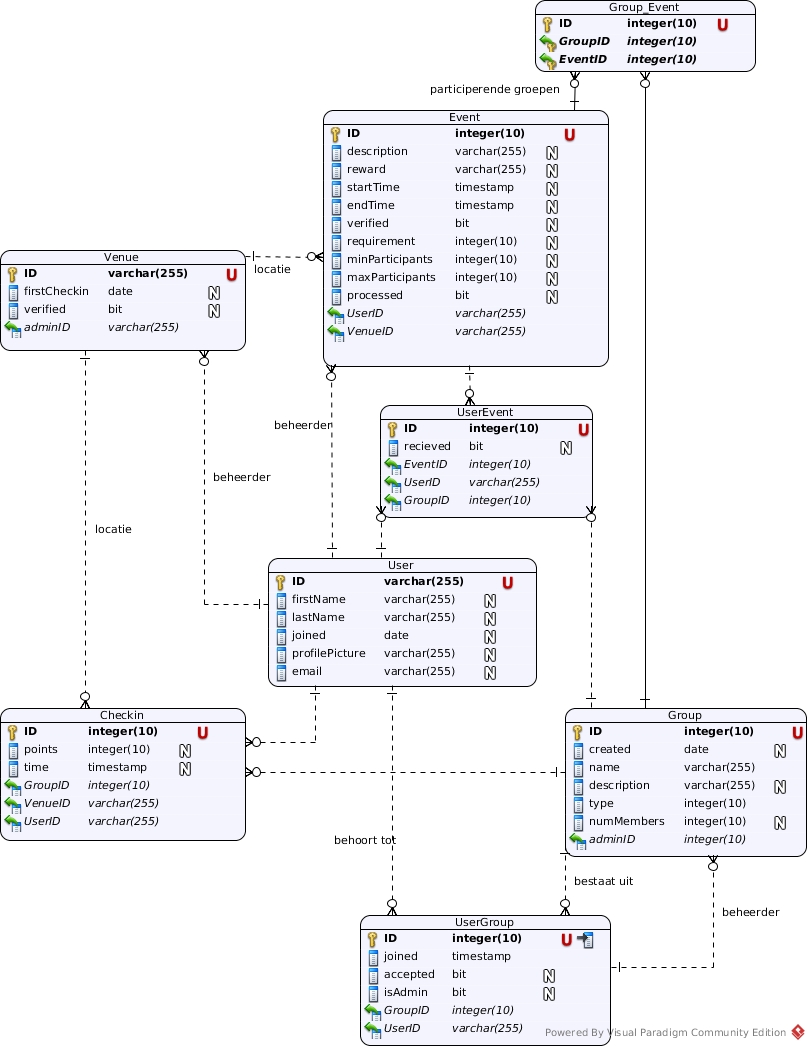
\includegraphics[scale=0.43]{backend_EER}
	\caption{Entity Relation diagram van de kern van de backend database}
	\label{fig:Backend ER}
\end{figure}

Figuur \ref{fig:Backend ER 2} toont het overige deel van de backend database. Wanneer een gebruiker zich voor het eerst authenticeert met de backend wordt er een SessionToken gekoppeld met de gebruiker. Deze token wordt meegegeven als parameter met iedere API call om de een gebruiker te authenticeren. 

De laatste tabel van de backend database houdt voor iedere gebruiker een gcmId bij. Deze ID wordt gebruikt voor de Google Cloud Messaging dienst.

\begin{figure}[H]
	\centering
	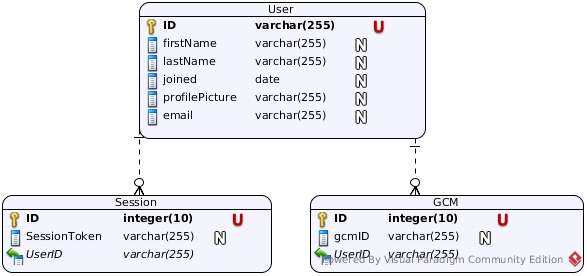
\includegraphics[scale=0.45]{backend_EER_deel2}
	\caption{Entity Relation diagram van het administratieve deel van de backend database}
	\label{fig:Backend ER 2}
\end{figure}

\subsubsection{backend API}
\label{backend API}
% generateRewards
De backend API bestaat uit een reeks methodes die kunnen opgeroepen worden vanop het mobiele toestel of vanop de webinterface. Dit is weergegeven met pijlen (3) en (5) op figuur \ref{fig:algemene structuur backend}. 

Een groot deel van de methodes hebben als doel het ophalen van gegevens uit de database, deze gegevens te mappen op een javaBean om vervolgens de bean terug te geven als resultaat. De voornaamste methodes van dit soort API calls zijn opgelijst in codefragment \ref{backend API}.


\begin{lstlisting}[caption={backend API methode signaturen ter opvraging van database informatie},label=lst:backend_api]
GroupsBean getAllGroups(String UserToken);
GroupsBean getGroupsForUser(String UserToken);
GroupBean getGroupInfo(String UserToken, long GroupId);
UsersBean getPendingRequest(String UserToken, long GroupId); 
	// geeft de lidmaatschapaanvragen van een groep terug

EventsBean getEventsForUser(String UserToken);
EventsBean getEventsForVenue(String UserToken, String VenueId);
RankingBean getRankingForEvent(String UserToken, long EventId);

VenueBean getVenueInfo(String UserToken, String VenueId);

UserBean getUserInfo(String UserToken);
OverviewBean getOverviewForUser(String UserToken);
\end{lstlisting}

Een tweede soort API calls wordt gebruikt om entiteiten van de tabellen Group, Event, UserGroup en UserEvent aan te maken of up te daten. De belangrijkste methode van dit soort is generateRewards(). De methode generateRewards() wordt vanuit een cronjob (zie sectie \ref{sec: GCE} Cron jobs) ieder kwartier opgeroepen. Prinicpieel werkt de functie als volgt:
\begin{enumerate}
  \item Controleert of er het afgelopen kwartier een event is beëindigd.
  \item Gaat voor elk beëndigd event bereken welke groepen gewonnen zijn a.d.h.v. de tijdstippen van de checkin entiteiten. Hierbij wordt er rekening gehouden met participatievoorwaarden zoals het minimaal en maximaal aantal leden van een groep.
  \item De leden van een winnende groep worden geplaast in de UserEvent tabel.
  \item Via het notificatiesysteem (zie sectie \ref{sec: GCE} Google Cloud Messaging) worden de winnende gebruikers verwittigd.
\end{enumerate}
Een beperking van dit systeem is dat een gebruiker gemiddeld 7,5 minuten moet wachten alvorens een notificatie van winst te ontvangen. Het is wel mogelijk de oproepfrequentie van de Cron job te verhogen.

Tot slot bevat de backend API nog methodes die gebruikers registeren, gebruikers authenticeren en communiceren met de GCM diensten. 

\subsection{Foursquare API}
\label{Foursquare API}

%Korte inleiding gebruik API
Zoals reeds eerder aangehaald maakt Triump gebruikt van locaties, deze locaties worden bekomen via de Foursquare API. De Foursquare API geeft de mogelijkheid aan ontwikkelaars om enorme gebruiker gegenereerde database van Foursquare te raadplegen. Naast locatie gegevens kan er ook informatie van gebruikers zoals namen geboortedata en profielfoto's opgevraagd worden.  Het mobiele toestel zal rechtstreeks requests sturen naar de foursquare API om bijvoorbeeld een lijst te krijgen van dichtbijzijnde locaties of om informatie van een locatie op te vragen. Het gebruik van de API wordt getoond in figuur \ref{fig:algemene structuur backend} pijl (1).

% Overzicht voor en nadelen gebruik API
Het werken met de API brengt echter wel nadelen met zich mee.
Allereerst wordt Triump hierdoor afhankelijk van een externe organisatie. Indien Foursquare beslist zijn open database te sluiten moet het ontwerp van Triump volledig herzien worden. Daarnaast wordt van commerciële applicaties verwacht dat ze reclame maken voor Foursquare door bijvoorbeeld het Foursquare logo op op te nemen in de layout.  Een tweede nadeel is dat de dataopslag verdeeld wordt over twee databases. Enerzijds de Google Cloud Datastore waar de data over groepen en checkins worden bijgehouden en anderzijds de Foursquare Datastore waar de locatie en gebruikergegevens zijn opgeslaan. Een laatste nadeel is dat locaties verplicht geregisteerd moeten zijn bij Foursquare teneinde zichtbaar te zijn op Triump. 

Indien locaties intern zouden aangemaakt en opgeslaan worden zouden de eerste twee nadelen verholpen zijn. 
Deze voor de hand liggende oplossing wordt echter niet toegepast aangezien dit zou impliceren dat Triump vanaf nul zijn locatiedatabase zou moeten vullen. Hierdoor zouden gebruikers ontmoedigd worden Triump boven Foursquare te kiezen. Daarnaast biedt Triump de optie een checkin door te propageren naar Foursquare waardoor we de functionaliteiten ervan uitbreiden. %dit is geen optie, maar altijd zo

Het laatste probleem wordt opgelost door het voorzien van een webinterface. Deze interface voorziet de mogelijkheid aan eigenaars van locaties om de nodige informatie omtrent hun café, zaak of restaurant zichtbaar te maken op Triump. Meer uitleg over de website volgt hieronder.

Er dient opgemerkt te worden dat Google met 'Google Places' gelijkaardige diensten biedt. Gebruik van deze API heeft dezelfde voor- en nadelen als de Foursquare API maar met de bijkomende beperking dat het aantal geregistreerde locaties veel kleiner is.


%werking API
Het mechanisme gebruik in de Foursquare API is zeer vanzelfsprekend. Alle gegevens, opgeslaan in de database, corresponeren met een RESTful (Representational State Transfer) Uniform Resource Locator (URL)  \cite{FS_API_website}. De frontend applicatie dient een connectie over HTTPS te starten met een Foursquare API Endpoint via de gewenste URL. Vervolgens zal de API Endpoint de gevraagde informatie in Javascript Object Notation (JSON) formaat terugzenden. JSON is een gestandaardiseerd gegevensformaat. JSON maakt gebruik van voor de mens leesbare tekst in de vorm van data-objecten die bestaan uit een of meer attributen met bijbehorende waarde. Het wordt hoofdzakelijk gebruikt voor uitwisseling van data tussen server en webapplicatie, als een alternatief voor xml. Het voordeel van JSON is de platformonafhankelijkheid \cite{JSON_def}. In listing ~\ref{lst:vb_foursquare_api} wordt een voorbeeld uitgewerkt waarbij de applicatie vanop de smartphone de informatie van een bepaalde locatie opvraagd.


\begin{lstlisting}[caption={Voorbeeld: werking Foursquare API},label=lst:vb_foursquare_api]

HTTPS connectie naar URL:
https://api.foursquare.com/v2/venues/4d972f73af3d236ad0561cc7?
	oauth_token=OMUUXC42I4GCMV3G21&v=20150101&m=foursquare

Antwoord:
"venue":
	{
	"id":"4d972f73af3d236ad0561cc7",
	"name":"POM D' API BRUXELLES",
	"contact":{},
	"location":
		{
		"address":"Koninginnegallerij",
		"lat":50.0,"lng":4.0,
		"postalCode":"1000",
		"city":"Brussels",
		"state":"Bruxelles-Capitale",
		"country":"Belgium",
		"formattedAddress":
		["Koninginnegallerij","1000 Brussels"]
		}
	}
\end{lstlisting}
 


\section{Frontend}
\subsection{Android applicatie}
\subsubsection{Waarom Android}
% Keuze android boven iOS
% 
Bij de ontwikkeling van de Triump applicatie is er gekozen voor Android als mobiel platform boven iOS of Windows Phone. Android heeft als voordeel dat het een groot marktaandeel heeft en er dus een groot publiek bereikt kan worden met de applicatie. Dit maakt dat Android als eerste platform de beste keuze is. De ontwikkeltools voor iOS en Windows Phone zijn ook niet cross-platform. Om apps te ontwikkelen voor iOS dient men over XCode te beschikken (enkel beschikbaar op Mac OS X) en om Windows Phone applicaties te ontwikkelen maakt men gebruik van Visual Studio (enkel beschikbaar op Windows). Vermits ons team bestaat uit 1 Windows, 1 Linux en 2 Mac gebruikers, was het dus een must om een cross-platform ontwikkelomgeving te hebben.
\subsubsection{Ontwikkelomgeving: Android Studio}
% vergelijking vs Eclipse
Vroeger was Eclipse de standaard ontwikkelomgeving (IDE) voor Android. Hierbij werd de standaard Eclipse installatie uitgebreid met de Android Developer Toolkit (ADT) plugin om Eclipse beter geschikt te maken voor Android Development. Op 16 mei 2013 stelde Google de nieuwste IDE voor Android voor: Android Studio. Deze IDE is gebaseerd op IntelliJ IDEA en biedt veel verbeteringen ten opzichte van Eclipse. In het begin waren er echter nog veel problemen met Android Studio waardoor veel mensen bij Eclipse bleven. Bij de aanvang van de ontwikkeling van Triump is er toch gekozen voor Android Studio omdat de meeste problemen toen reeds opgelost waren.
De voordelen van Android Studio waren dan ook overduidelijk. Betere code generatie en auto-complete dan Eclipse, zeer goede integratie met de Android SDK en live previews in de layout builder. 

\begin{figure}[H]
	\centering
	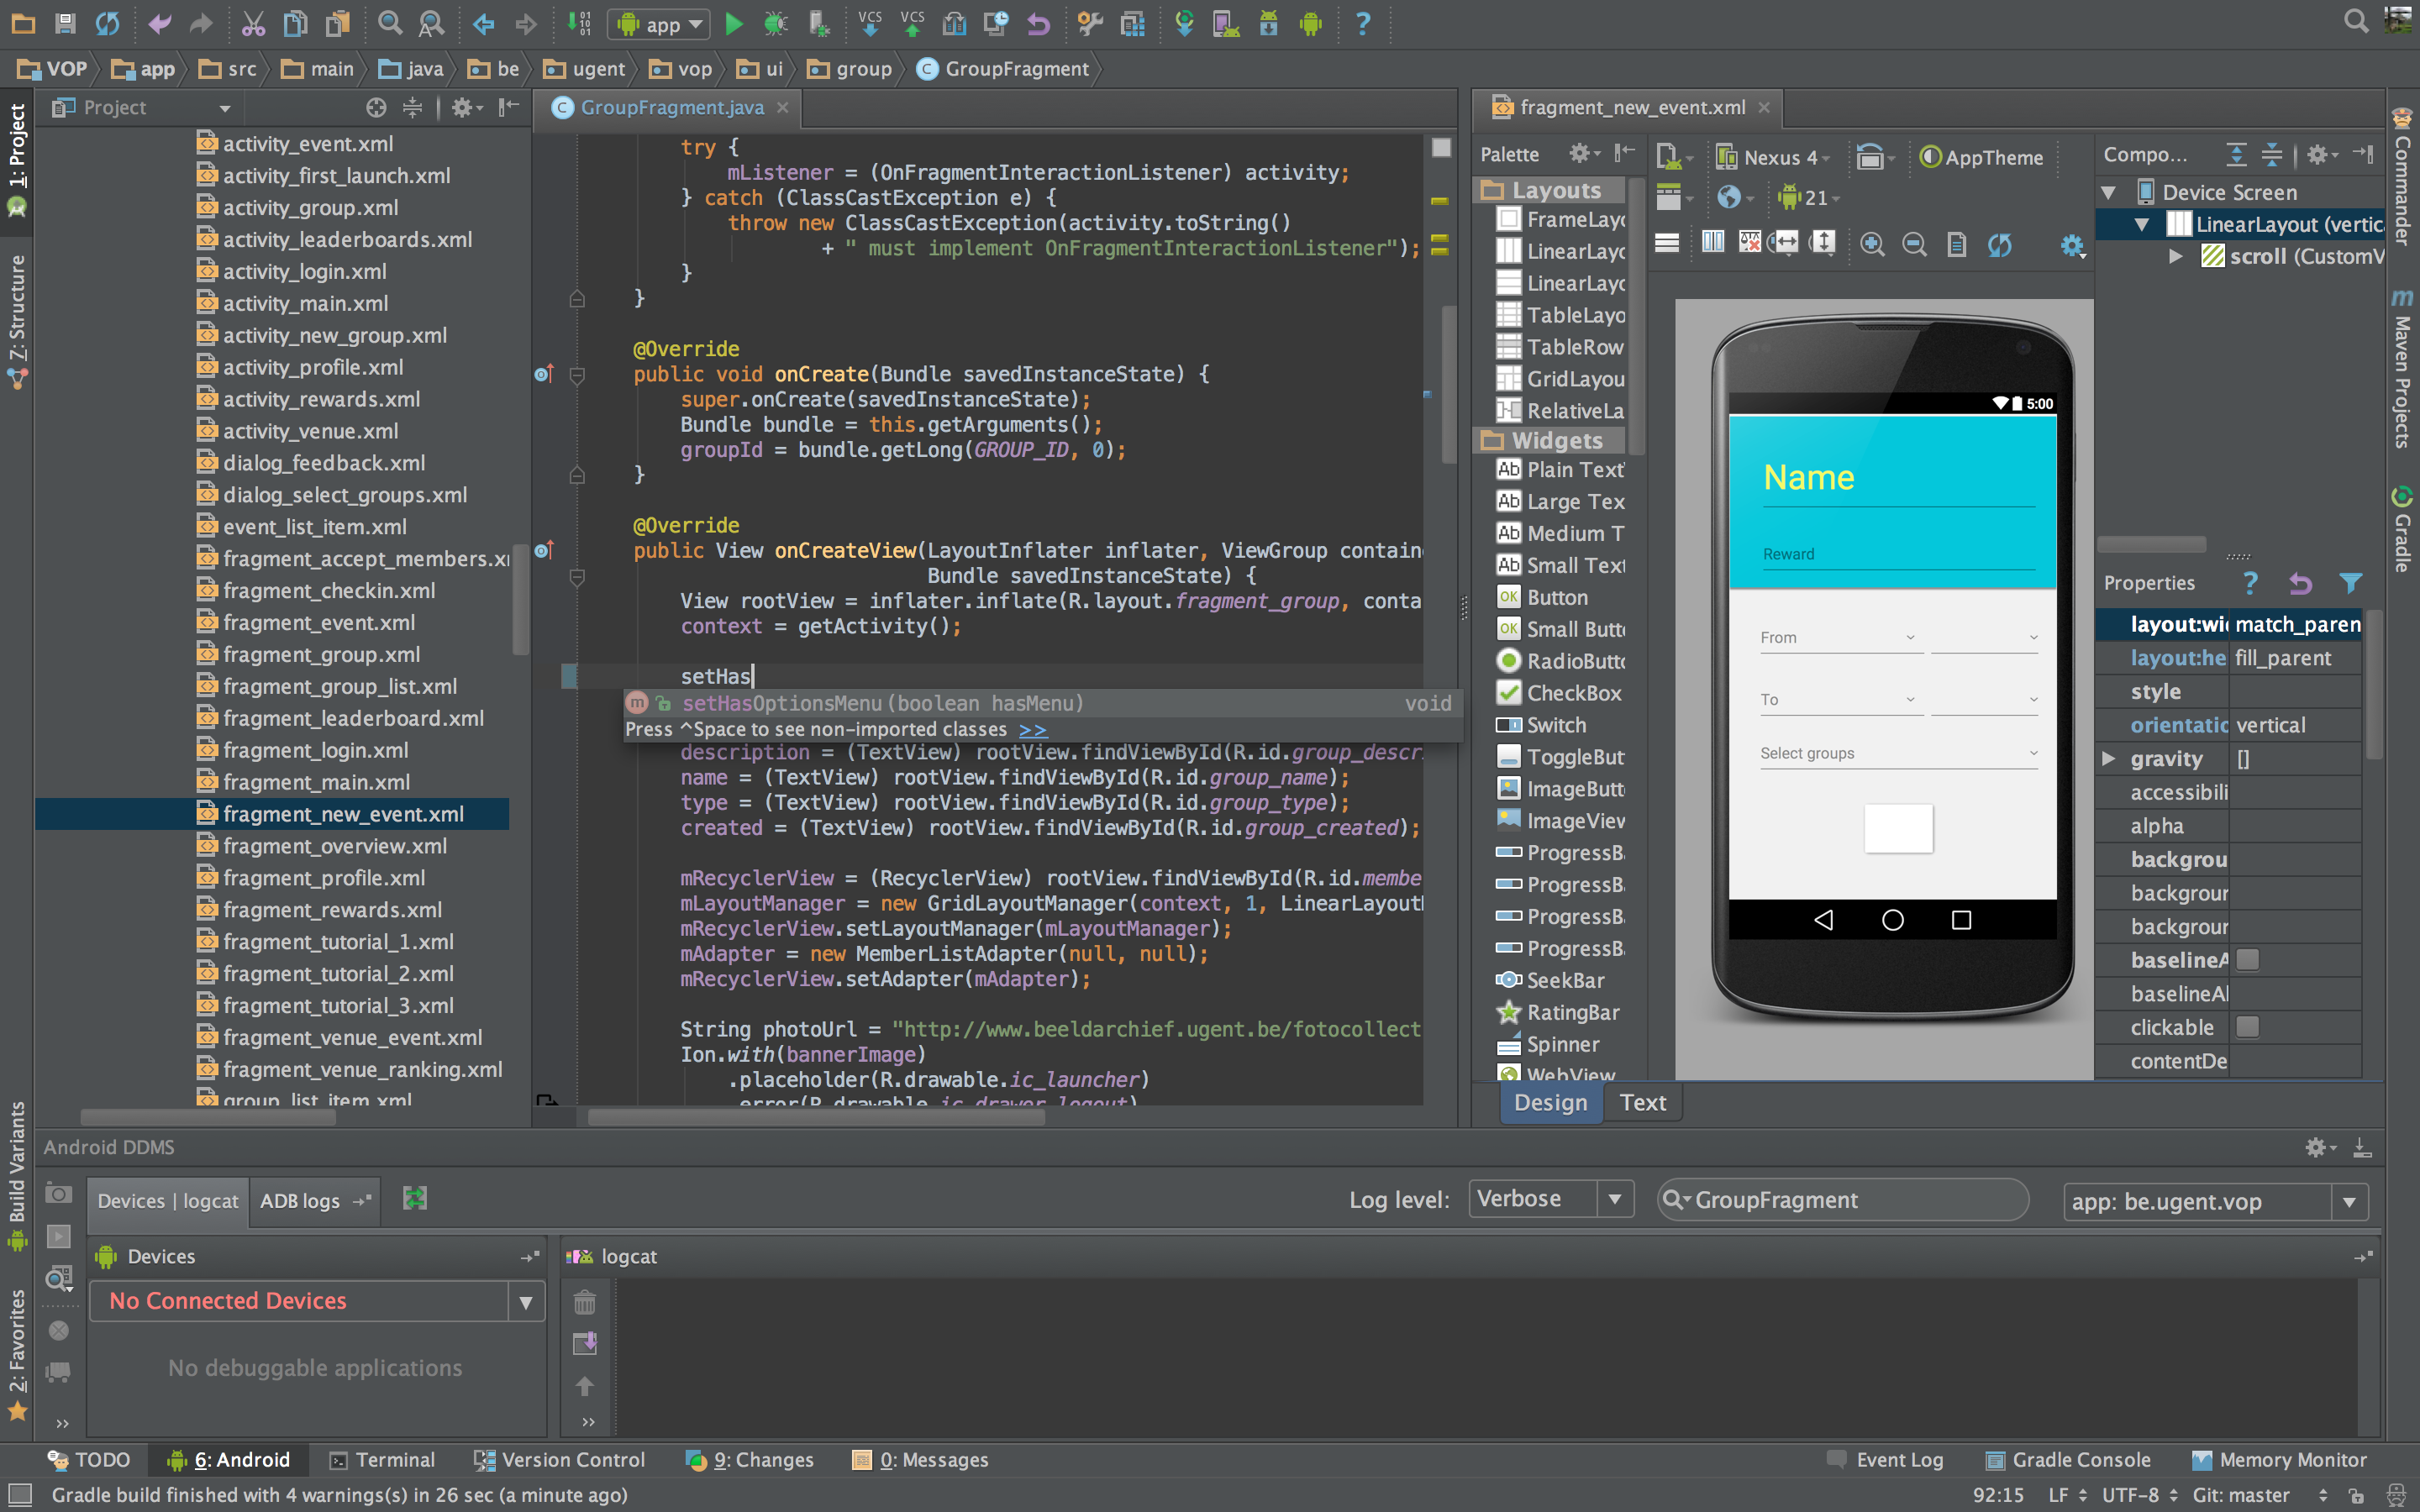
\includegraphics[width=\linewidth]{android_studio}
	\caption{Een typische workflow in Android Studio}
	\label{fig:Android Studio Workflow}
\end{figure}

\subsubsection{Ontwerpkeuzes}
Tijdens de ontwikkeling van Triump is er voor gekozen om te werken met de laatste nieuwe technologieën. Dat wil zeggen dat Triump ontwikkelt is met als doel volledig compatibel te zijn met de laatste versie van Android: 5.1 Lollipop. Triump is daarnaast wel nog steeds compatibel met alle Android versies vanaf 4.1 Jelly Bean. Hierdoor bereikt de app 87,5\% van alle Android toestellen \cite{market_share}. Oudere versies zullen niet ondersteund worden vermits deze slechts 12,5\% marktaandeel hebben en het te veel moeite zou kosten om te zorgen dat Triump ook op deze versies correct werkt en uitvoerig getest is.
Android development gebeurd in Java, maar er zijn enkele Android-specifieke ontwerppatronen waarvan we gebruik gemaakt hebben. Onder andere voor het asynchroon laden van informatie, het opslaan van data en het opbouwen van efficiënte UI lijsten zijn er speciale ontwerppatronen in Android. Deze zullen in de volgende secties verder uitgelegd worden.

\subsubsection{Material Design}
Triump is ontwikkeld voor Android Lollopop. Dit houdt in dat er gebruik gemaakt wordt van de Material Design Guidelines \cite{Material_Design}. Door de Material Design Guidelines te volgen is het makkelijker om een consistent look-and-feel te verkrijgen in de app die volledig in lijn ligt met de rest van het Android ecosysteem.
Om de correcte implementatie van Material Design te garanderen, is er gebruik gemaakt van enkele externe bibliotheken. Deze bibliotheken bieden extra functionaliteit ten opzichte van de standaard Android API waardoor het makkelijker is het correcte design te verkrijgen. Deze bibliotheken zijn ook altijd backwards compatible met versies van Android lager dan Lollipop. Hierdoor wordt er een uniforme look verkregen op alle versies die de app ondersteunt.
De gebruikt bibliotheken om Material Design te implementeren zijn:
\begin{description}
\item[Material Design Library \cite{navasmdc}] Een bibliotheek die verschillende UI componenten bevat die voldoen aan de Material Design Guidelines zoals de Flat Buttons, Progress Bar Indicators en Switches.
\item[FloatingActionButton \cite{floatingactionbutton}] Een bibliotheek die de Floating Action Button van de Material Design Specification implementeert en toelaat om die toe te voegen aan een RecyclerView (zie verder).
\item[MaterialEditText \cite{materialedittext}] Een bibliotheek die een consistent implementatie biedt voor tekstvelden in formulieren. De bibliotheek voorziet verschillende functies voor de tekstvelden zoals maximum lengte, hints, iconen en aangepaste kleuren.
\end{description}

\subsubsection{RecyclerView}
Sinds Android 5.0 is er een nieuwe manier geïntroduceerd om lijsten weer te geven in de UI van de applicatie. Deze nieuwe widget (zo heten de UI componenten in Android) is de RecyclerView. De RecyclerView vervangt de oudere ListView widget. Om de voordelen van de RecyclerView uit te leggen moet men eerst de concepten van Android begrijpen.
De ListView en RecyclerView geven beiden een lijst weer van data. Beide widgets worden aangestuurd door een zogenaamde Adapter. Die Adapter is een speciale klasse die de widgets oproepen om te rijen van de lijsten te vullen met data. Daarvoor moet de Adapter bepaalde methoden implementeren die dan door de ListView / RecyclerView opgeroepen worden. Bij zowel ListView als RecyclerView is 1 van die methodes verantwoordelijk voor het vullen dan de View van 1 rij met de correcte data.
Voor elke rij in de lijst is de layout namelijk vastgelegd in een XML bestand. Aan de hand van dat XML bestand wordt dan voor elke rij een View object aangemaakt dat de correcte layout bevat voor die rij. Op dat moment is het View object voor die rij nog niet gevuld met de correcte data. Daarvoor wordt bij de Adapter een methode opgeroepen om die View te vullen met de correcte data.
Het is in deze stap dat RecyclerView en ListView fundamenteel verschillen. In het geval van een ListView zal de Adapter voor elke rij verschillende findViewById(int id) operaties moeten doen om de correcte sub-View van de View van de rij te verkrijgen. Dat is nodig omdat de Adapter een referentie moet verkrijgen naar bijvoorbeeld een label View binnen de View van de rij. Deze findViewById(int id) operaties zijn echter zeer cpu-intensief. Hierdoor is scrollen in traditionele ListViews niet zo vloeiend.
RecyclerView maakt het grootste deel van de findViewById(int id) operaties overbodig door standaard gebruik te maken het ViewHolder patroon.

% Nog meer uitleg over ViewHolder bij schrijven...

\subsubsection{Loaders}
In Android gebeurd het tekenen en het interageren met de UI, net zoals bij de meeste andere GUI toolkits op de main thread. Dit betekent dat het inladen van data over bijvoorbeeld het netwerk of van de lokale opslag in een aparte thread moeten gebeuren. Is dit niet het geval, dan zal de volledige UI van de applicatie vast hangen tijdens het ophalen van de data. Dat is natuurlijk niet wenselijk vermits dit een slechte User Experience geeft.
Daarom bevat Android het concept van Loaders. De bedoeling van Loaders is om data op een asynchrone manier in te laden (dus op een aparte thread) en de resultaten via een callback terug te sturen naar de main UI thread waar de resultaten dan getoond kunnen worden op het scherm. 

\subsubsection{Inloggen en authenticatie via Foursquare}

% Recycler view, nieuwste trends
% material design: welke lib. dat we gebruikt hebben
% Loadermechanismen
% Lokale SQLite DB
% Cardmechanisme

\subsection{Webinterface}
\subsubsection{Doel}
% De Waarom Vraag => !! zou dit niet beter eerder in het verslag al worden gezegd? !!
Voor een aantal taken is een smartphone niet helemaal geschikt. Deze heeft een klein scherm en de touchbediening is niet altijd handig. Zulke taken zijn het beheren van groepen en het aanmaken van promoties.
Deze taken worden met bepaalde regelmaat gebeuren en zijn gemakkelijker op een groter scherm uit te voeren. Specifieke gebruikers, zoals uitbaters van locaties die een promotie willen opzetten om zo klanten te lokken, zullen deze taken willen uitvoeren. Daarom is Triump uitgebreid met een webinterface.
Onze site zal tevens dienst doen als infopunt voor huidige en toekomstige gebruikers. Op de site staat informatie over het doel en de meerwaarde van Triump, en wordt er een link voorzien zodat toekomstige gebruikers de applicatie kunnen downloaden.\\
Op onze website kunnen gebruikers net als in de android-applicatie inloggen met Foursquare. Het is de bedoeling dat het registereren van een Foursquare-locatie steeds via de website gebeurd, net als het aanmaken van promoties door een eigenaar van een registreerde locatie. Het opleggen van registratie van een locatie door de eigenaar ervan moet ervoor zorgen dat er geen valse promoties worden opgezet. Zonder registratie zou immers iemand een promotie kunnen aanmaken voor een bepaalde locatie zonder dat deze ook daadwerkelijk wordt gegeven. Dit zou Triump een stuk minder aantrekkelijk maken voor de gebruiker.

\subsubsection{Django-framework}
Bij het maken van een website kan men verschillende keuzes maken.
Eerst en vooral is er de keuze of er gebruik wordt gemaakt van een bestaand framework, zoals Ruby on Rails, ASP.NET en Django, of dat men zelf de nodige functionaliteit implementeert met bijvoorbeeld PHP.
Omdat de webinterface slechts extra functionaliteit mogelijk maakt en dus niet het grootste deel van ons project is, werd besloten om deze voorlopig niet te uitgebreid te maken.
Het helemaal zelf opbouwen van de site is daarom een slecht idee: bestaande frameworks bieden ruim voldoende functionaliteit aan om onze website te maken. De frameworks zijn daarboven reeds geoptimaliseerd en bevatten functies zoals een standaardmanier om gebruikers veilig in te loggen. Het inloggen helemaal zelf implementeren daarintegen zou veel tijd en werk vragen, terwijl de kwaliteit naar alle waarschijnlijkheid beneden die van bestaande oplossingen zou liggen. 
Daarnaast moet men nog kiezen om ofwel de site bij een hosting-dienst te plaatsen, ofwel zelf de site te hosten op een eigen pc. De hosting zelf voorzien brengt vele moeilijkheden met zich mee: liefst wordt er gewerkt met een vast IP-adres, maar providers kennen aan gewone klanten slechts een tijdelijk IP-adres toe. Daarboven dient men dan ook de DNS-servers (minmaal 2) zelf te verzorgen.
De andere oplossing, gebruik maken van een hosting-dienst, is veel eenvoudiger. Voor een vast bedrag, per maand of jaar, wordt de website geplaatst op de servers van de hosting-dienst. Deze neemt extra moeilijkheden, zoals het instellen en onderhouden van DNS-servers op zich.
Het databasemanagment systeem (DBMS) moet ook nog worden gekozen indien dit van toepassing is. Hier was dit het geval: op de site worden gebruikers aangemaakt waarbij bepaalde informatie wordt opgeslaan, zoals hun Foursquare-identiteit, zodat de gebruiker maar 1 keer met Foursquare moet inloggen. \\
\begin{figure}[H]
	\centering
	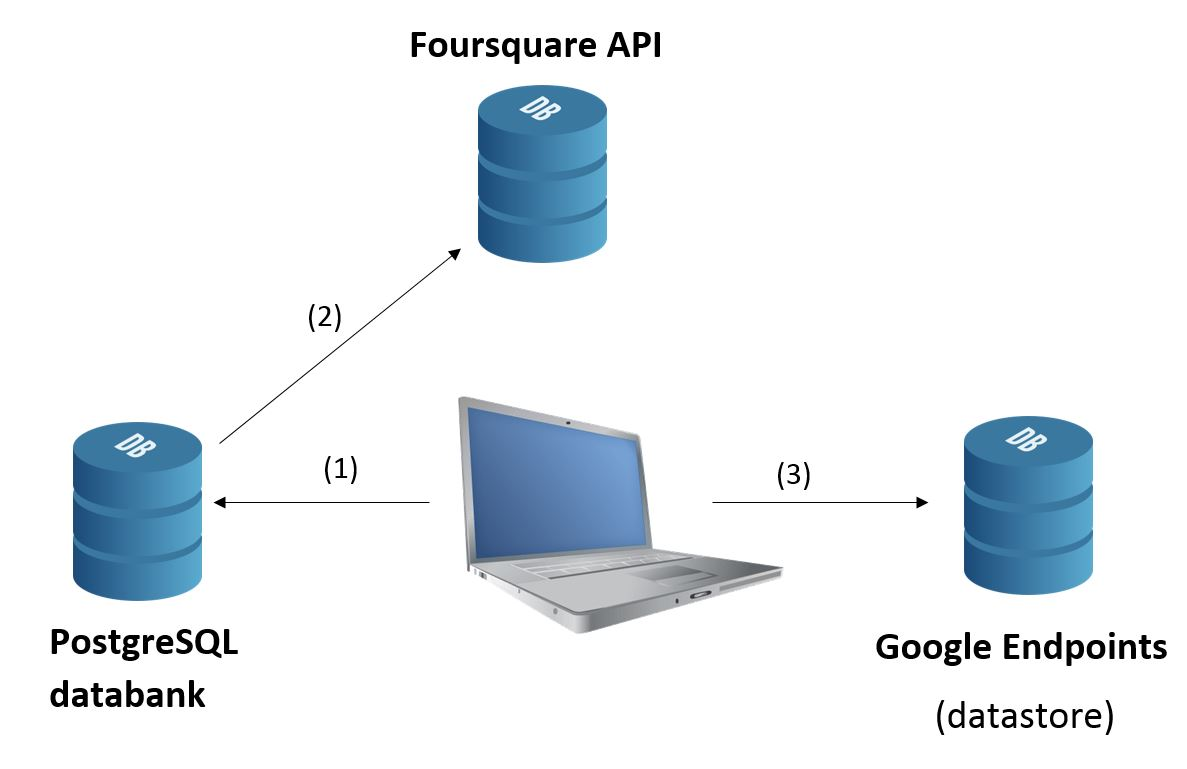
\includegraphics[scale=0.25]{webinterface_structuur}
	\caption{Werking webinterface}
	\label{fig:Webinterface}
\end{figure}
Als framework voor de webinterface werd gekozen voor Django. Dit framework maakt gebruik van de taal Python: een eenvoudig, maar krachtig taal. Django maakt het mogelijk om op relatief korte tijd toch een dynamische website te bouwen. Bij een dynamische website wordt de HTML-pagina die door de gebruiker wordt opgevraagd op het moment zelf door de server gegenereerd. Dit gebeurt door informatie uit bijvoorbeeld een databank op te halen, in ons geval de GCE backend, en dan een HTML-template in te vullen met deze informatie. Hierin ligt het verschil met statische websites, waar iedere gebruiker dezelfde vaste HTML-pagina's te zien krijgt.
Een voordeel van het werken met Django is dat er hosting-diensten bestaan die zich specialiseren in het hosten van Django-projecten. Wij kozen voor zo een dienst, namelijk http://djangoeurope.com.
Bij deze dienst was er de mogelijkheid te kiezen uit verschillende databasemanagment systemen. Er werd gekozen voor PostgreSQL: een open source DBMS waar wij reeds mee hebben gewerkt tijdens het vak "Databanken".
De manier waarop er wordt gewerkt wordt weergegeven in \ref{fig:Webinterface}. Men kan zien dat de server die de website host geconnecteerd is met een PostgreSQL databank (pijl 1). Deze maakt het mogelijk om gebruikers te laten inloggen met een eigen account, waarbij men dan extra data kan opslaan. Er werd reeds aangehaald dat gebruikers ook hier met Foursquare dienen in te loggen, dit gebeurt na het registreren. Zoals te zien op de figuur gebeurt alle communicatie met de Foursquare API vanop de webserver (pijl 2), niet door de computer van de gebruiker. Deze communicatie omvat het ophalen van gegevens van de gebruiker en locaties uit de databank van Foursquare.
Op de figuur kan men ook zien dat er vanop de computer van de gebruiker wordt gecommuniceerd met de centrale backend van Triump.
Deze communicatie verloopt via Javascript en dient om bijvoorbeeld het organiseren van een evenement mogelijk te maken.
De keuze voor Javascript is vooral gemotiveerd door de eenvoud van dit alternatief. Google biedt namelijk een API aan die het mogelijk maakt om Google Endpoints via Javascript aan te spreken.
Zo wordt gemakkelijk een van de functies uit de backend opgeroepen en kan het resultaat, dat in JSON wordt ontvangen, ook vlot worden verwerkt met behulp van Javascript.
Deze keuze brengt wel nadelen met zich mee. Aan de basis van deze nadelen ligt het feit dat Javascript op de computer van de gebruiker wordt uitgevoerd, en niet op de server die de website host. 
Javascript is alomtegenwoordig, mmar toch zijn er computers waarop, bewust of onbewust, Javascript niet is geïnstalleerd of uitgeschakeld. 
Deze computers kunnen dan weinig aanvangen met de webinterface, die afhangt van de Javascript-code. Dit probleem werd aangepakt door op de website te vermelden dat Javascript noodzakelijk is om een goede werking te verzekeren.
Het 'client-side' uitvoeren van code brengt nog een ander nadeel met zich mee: het vormt namelijk een zwak punt in de verdediging tegen aanvallen van buitenaf.
Aangezien personen met slechte bedoelingen de code kunnen bestuderen en niet enkel het antwoord te zien krijgen, verhoogt de kans dat men de website kan saboteren, gegevens kan stelen,...
Een alternatief is het gebruiken van een python-module op de webserver die communicatie met Google Endpoints mogelijk maakt. Dit zou ten goede komen, aangezien de code 'server-side' wordt uitgevoerd.
Het legt echter wel meer belasting op de server die de website host, deze neemt dan alle communicatie, voor alle gebruikers, met de Triump backend voor zijn rekening.
Voorlopig, tijdens de testfase, kan men aannemen dat Triump geen doelwit zal worden van hackers en kan gewoon met Javascript worden gewerkt. Later, bij verdere uitwerking van Triump, kan de site nog altijd worden aangepast.
(TODO: hoe gebeurt registratie
	   andere mogelijkheden van de webinterface) 

